\documentclass[final]{beamer}
\usepackage[T1]{fontenc}
\usepackage{pslatex}
\usepackage{setspace}
\usepackage{color}
\usepackage{tikz}
\usepackage{pdfpages}
\usetikzlibrary{arrows,shapes,shapes.multipart,matrix,positioning,shadows,calc}
%\usepackage[size=custom,width=153,height=102,scale=1.2]{beamerposter}
%\providecommand\thispdfpagelabel[1]{}

\mode<presentation> {
	\usetheme{Frankfurt}
	\usecolortheme{seahorse}
}

\tikzstyle{uiformat} = [rectangle, draw, thin, fill=orange!20]
\tikzstyle{servformat} = [rectangle, draw, thin, fill=blue!20]
\tikzstyle{dbformat} = [ellipse, draw, thin, fill=green!20]

\title[PLM] % (optional, only for long titles)
{Project Lifecycle Management}
\subtitle{Iteration 2}
\author[] % (optional, for multiple authors)
{Alan, Christian, Manav, Rachit, Tandhy, Vipul, Yuvaraj}
\date[November 7, 2013] % (optional)
{November 7, 2013}

\setbeamertemplate{frametitle in sidebar}[shaded]

\begin{document}
\begin{frame}
	\titlepage
\end{frame}

%%%%%%%%
\section{Requirement Analysis}

\begin{frame}
	\frametitle{Minimum Requirements}
	\begin{beamerboxesrounded}[shadow]{}
		\begin{itemize}
			\item{Register}
			\item{Login}
			\item{Manage project}
			\item{Manage iteration}
			\item{Manage user story}
			\item{Manage task}
		\end{itemize}
	\end{beamerboxesrounded}
\end{frame}

\begin{frame}
	\frametitle{User Stories This Iteration}
	\begin{beamerboxesrounded}[shadow]{Project}
		Create, Update, View projects
	\end{beamerboxesrounded}

	\begin{beamerboxesrounded}[shadow]{Iteration}
		Create, Update, View iterations under a project
	\end{beamerboxesrounded}

	\begin{beamerboxesrounded}[shadow]{User Story}
		Create, Update, View user stories under an iteration
	\end{beamerboxesrounded}

	\begin{beamerboxesrounded}[shadow]{Task}
		Create, Update, View tasks under a user story
	\end{beamerboxesrounded}
\end{frame}

%%%%%%%%
\section{Architecture}

\begin{frame}
	\frametitle{Software Architecture}
	%\begin{figure}
	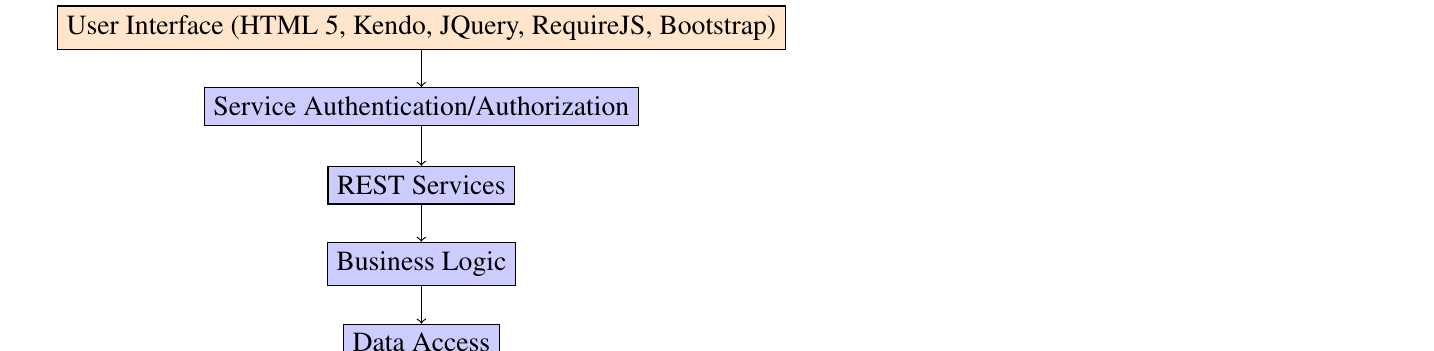
\begin{tikzpicture}[scale=1.25]
		\path[use as bounding box] (-4,-3) rectangle (10,0);
		\path[->]<1-> node[uiformat] (ui) {User Interface (HTML 5, Kendo, JQuery, RequireJS, Bootstrap)};
		\path[->]<1-> node[servformat, below of=ui] (auth) {Service Authentication/Authorization}
			(ui) edge node {} (auth);
		\path[->]<1-> node[servformat, below of=auth] (rest) {REST Services}
			(auth) edge node {} (rest);
		\path[->]<1-> node[servformat, below of=rest] (logic) {Business Logic}
			(rest) edge node {} (logic);
		\path[->]<1-> node[servformat, below of=logic] (dao) {Data Access}
			(logic) edge node {} (dao);
		\path[->]<1-> node[dbformat, below of=dao] (db) {MySQL Database}
			(dao) edge node {} (db);
		%\path[->, draw]<1-> (rest) -- +(0,1) -| node[near start] {} (dao);
	\end{tikzpicture}
	%\end{figure}
\end{frame}

\begin{frame}
	\frametitle{Software Architecture}

	\begin{beamerboxesrounded}[shadow]{User Interface}
		\begin{itemize}
			\item{Model View View Model (MVVM) pattern}
			\item{MVVM separates UI and back end}
			\item{Kendo framework (JQuery library) used for MVVM}
		\end{itemize}
	\end{beamerboxesrounded}

	\begin{beamerboxesrounded}[shadow]{Service}
		\begin{itemize}
			\item{Tiered architecture}
			\item{Authentication
				\begin{itemize}
					\item{username and password $\rightarrow$ session token}
				\end{itemize}
			}
			\item{Authorization 
				\begin{itemize}
					\item{session token and project ID $\rightarrow$ access granted/denied}
				\end{itemize}
			}
			\item{Business layer, Data access layer, Database layer}
		\end{itemize}
	\end{beamerboxesrounded}
\end{frame}

%%%%%%%%%
\section{Design}

\begin{frame}
	\frametitle{Database Design}
	%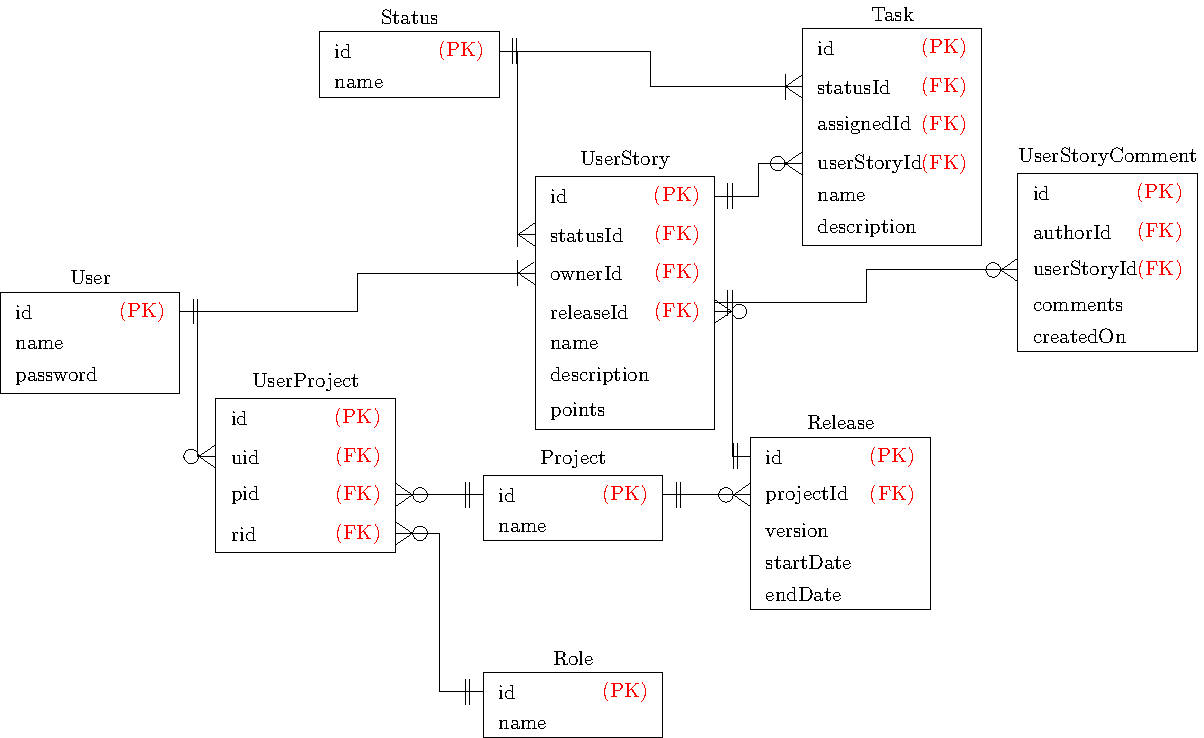
\includepdf{database.pdf}
	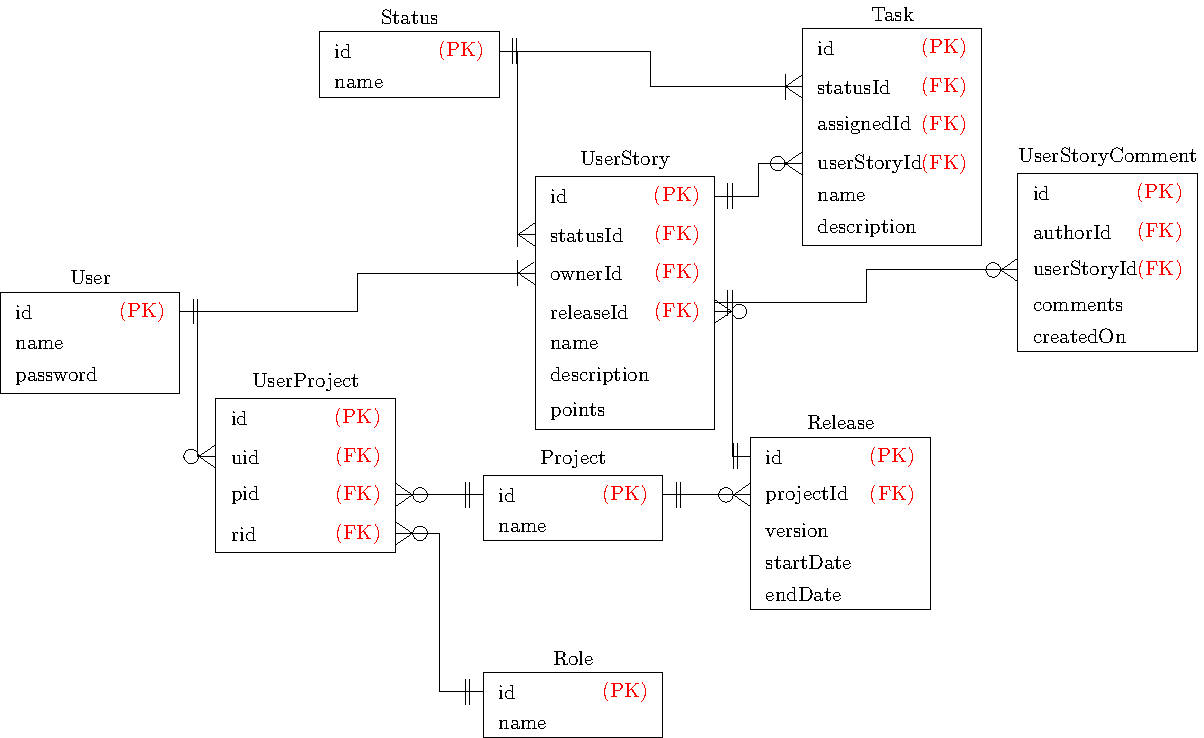
\includegraphics[width = 0.9\textwidth]{./database}
\end{frame}

\begin{frame}
	\frametitle{Class Diagram}
	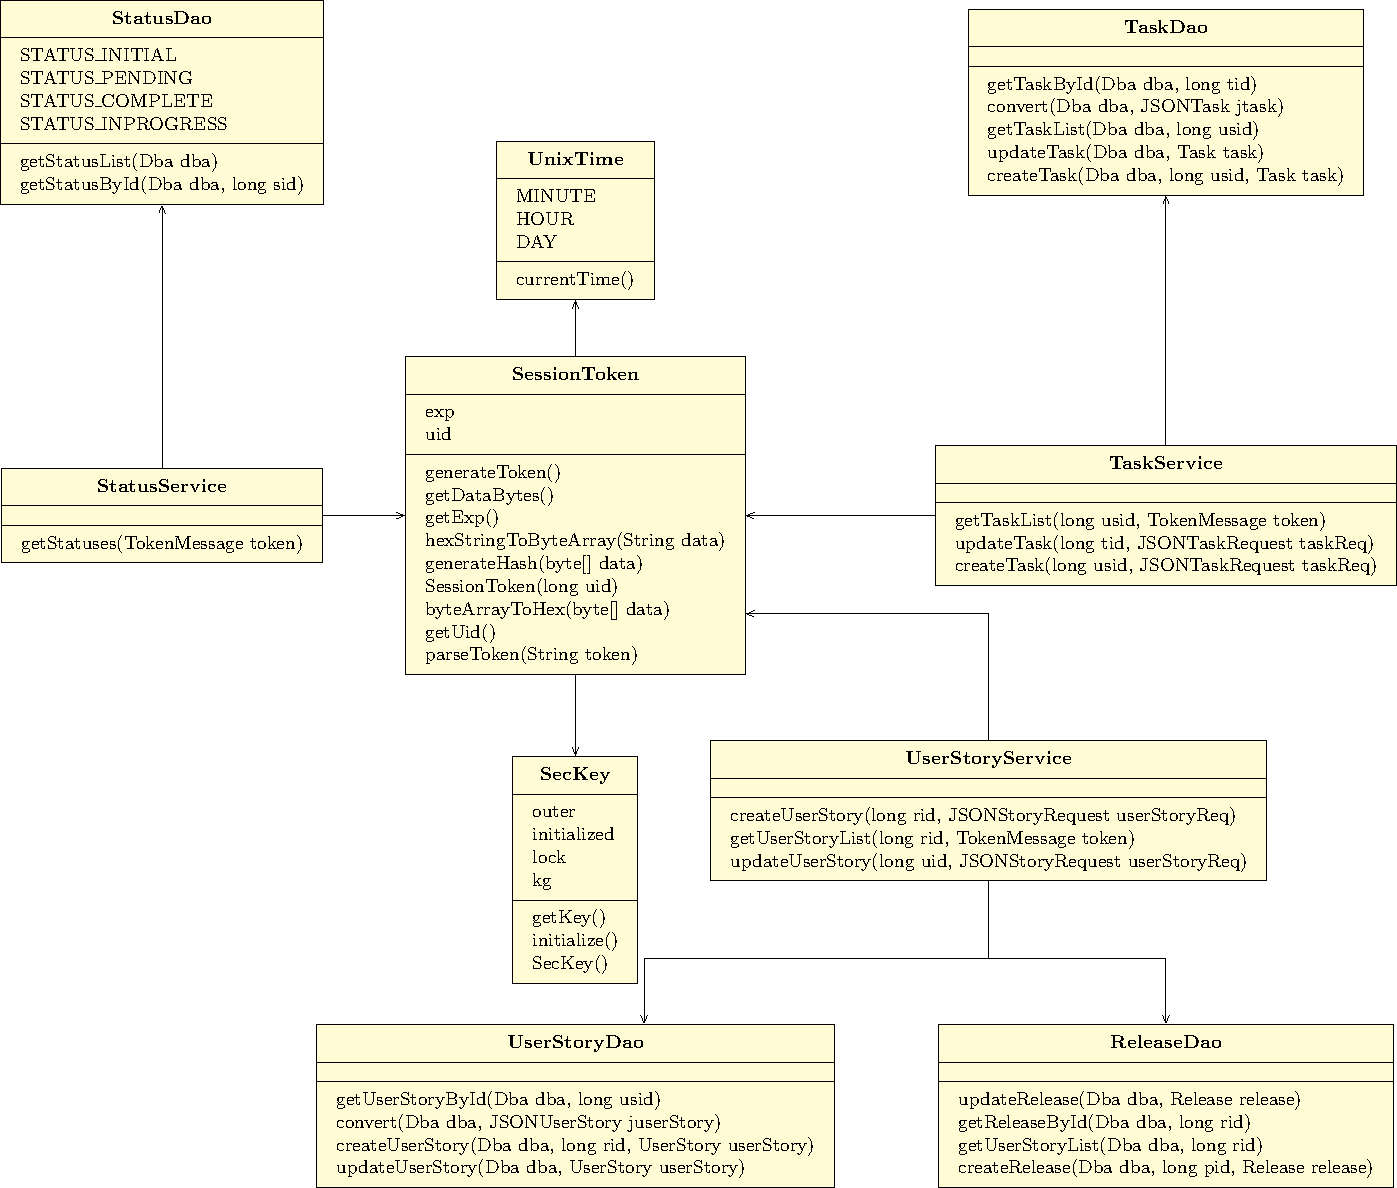
\includegraphics[width = 0.8\textwidth]{./classdiagram-presentation}
\end{frame}


%%%%%%%%%
\section{Implementation}

\begin{frame}
	\frametitle{Development Tools Used}
	\begin{beamerboxesrounded}[shadow]{}
		\begin{itemize}
			\item{Git / GitHub for version control and issue tracking}
			\item{Pivotal Tracker for requirement analysis}
			\item{Google Group for communication}
			\item{JUnit for service testing}
			\item{Selenium for UI testing}
		\end{itemize}
	\end{beamerboxesrounded}
\end{frame}

\begin{frame}
	\frametitle{Deployment Tools Used}
	\begin{beamerboxesrounded}[shadow]{}
		\begin{itemize}
			\item{Apache Tomcat}
			\item{Apache Ant}
			\item{MySQL}
		\end{itemize}
	\end{beamerboxesrounded}
\end{frame}


%%%%%%%%%
\section{Testing}

\begin{frame}
	\frametitle{Service Testing}
	\begin{beamerboxesrounded}[shadow]{Unit Testing for Business Logic}
		\begin{itemize}
			\item{Permissions -- Passed}
			\item{Session Tokens -- Passed}
		\end{itemize}
	\end{beamerboxesrounded}

	\begin{beamerboxesrounded}[shadow]{Integration Testing for REST Services}
		\begin{itemize}
			\item{Project -- Passed}
			\item{Iteration -- Passed}
			\item{Status (user story and task) -- Passed}
			\item{Task -- Passed}
			\item{User Story -- Passed}
		\end{itemize}
	\end{beamerboxesrounded}
\end{frame}

%\begin{frame}
	%\frametitle{UI Testing}
	%\begin{beamerboxesrounded}[shadow]{}
		%\begin{itemize}
			%\item{Fill in this stuff}
		%\end{itemize}
	%\end{beamerboxesrounded}
%\end{frame}


%%%%%%%%%
\section{Project Management}

\begin{frame}
	\frametitle{Metrics}
	\begin{beamerboxesrounded}[shadow]{Service Code}
		This Iteration:
		\begin{itemize}
			\item{38 files changed}
			\item{2462 insertions}
			\item{55 deletions}
		\end{itemize}

		Total:
		\begin{itemize}
			\item{69 files}
			\item{6383 lines of code}
		\end{itemize}
	\end{beamerboxesrounded}
\end{frame}

\begin{frame}
	\frametitle{Metrics}
	\begin{beamerboxesrounded}[shadow]{UI Code}
		This Iteration:
		\begin{itemize}
			\item{13 files changed}
			\item{2501 insertions}
			\item{6 deletions}
		\end{itemize}

		Total:
		\begin{itemize}
			\item{118 files}
			\item{7953 lines of code}
		\end{itemize}
	\end{beamerboxesrounded}
\end{frame}

\begin{frame}
	\frametitle{Metrics}
	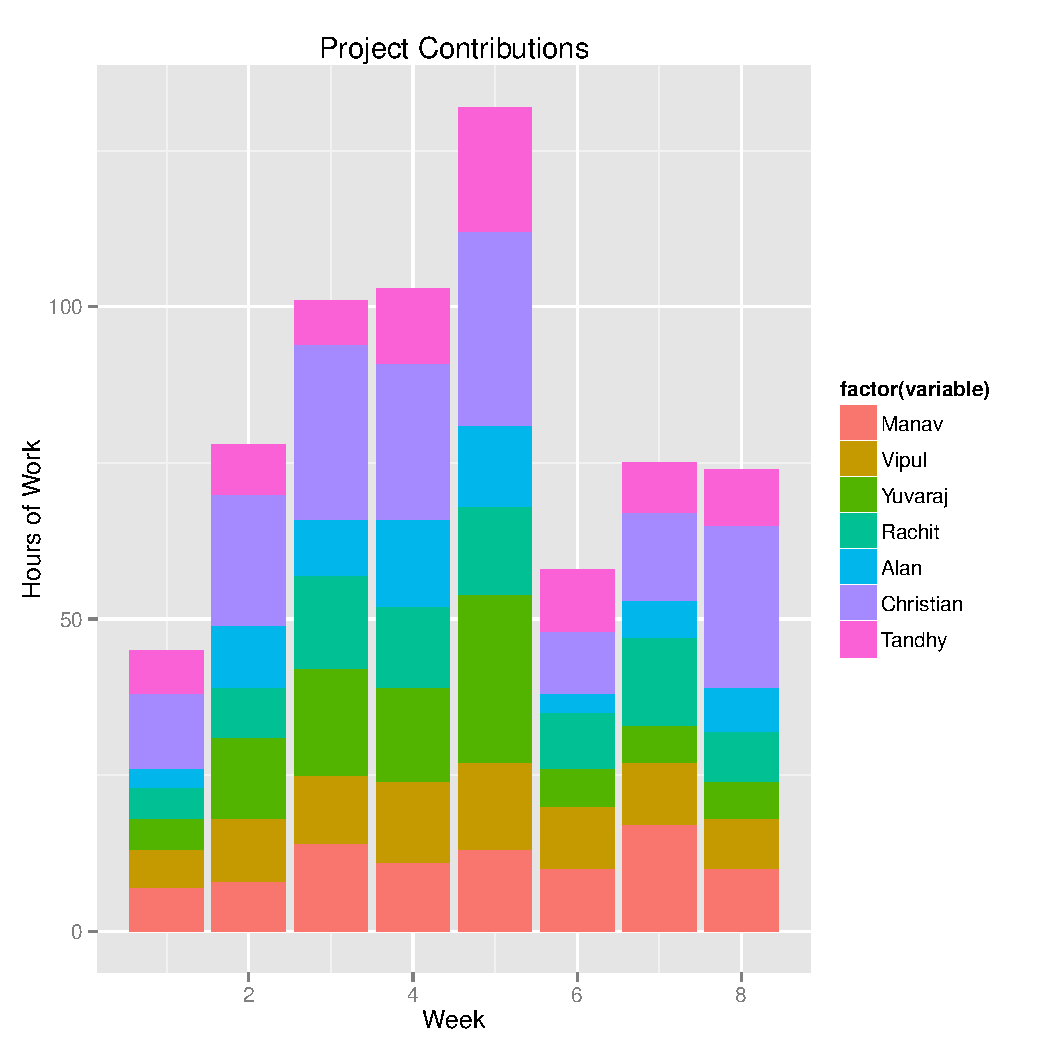
\includegraphics[width = 0.7\textwidth]{./hours_worked}
\end{frame}

%%%%%%%%%
\section{Conclusions}

\begin{frame}
	\frametitle{Current Progress}
	\begin{beamerboxesrounded}[shadow]{Minimum Functionality Revisited}
		\begin{itemize}
			\item{Register -- Done}
			\item{Login -- Done}
			\item{Manage projects -- Needs user management}
			\item{Create iterations -- Done}
			\item{Manage user stories -- Done}
			\item{Manage tasks -- Done}
		\end{itemize}
	\end{beamerboxesrounded}
\end{frame}

\begin{frame}
	\frametitle{Lessons Learned}
	\begin{beamerboxesrounded}[shadow]{}
		\begin{itemize}
			\item{Communication}
			\item{Steady progress across the iteration}
		\end{itemize}
	\end{beamerboxesrounded}
\end{frame}

\begin{frame}
	\frametitle{Future Work}
	\begin{beamerboxesrounded}[shadow]{}
		\begin{itemize}
			\item{Adding users to projects}
			\item{Migrating user stories to different iterations}
			\item{Generating reports}
		\end{itemize}
	\end{beamerboxesrounded}
\end{frame}

\end{document}
